\textbf{\chapter{Implementación y Experimentos}}
\section{Diseño experimental}
El procedimiento experimental consiste en entrenar
un modelo de aprendizaje profundo capaz de estimar la
altura de objetos y comparar sus predicciones frente al método de calibración manual de cámara y reproyección geométrica.
En la Tabla~\ref{tab:ExperimentsSummary} se muestran los diferentes métodos a comparar en esta sección.
El código desarrollado se encuentra disponible en el GitHub \code{https://github.com/briansenas/TFM_SVMIW}.
La evaluación de la implementación propuesta se ha realizado tomando como referencia tanto los resultados publicados en el
trabajo original~\cite{SVMIW} como los obtenidos posteriormente en~\cite{SPEC}.
\par
Para ello, el modelo se entrena con la misma partición
de entrenamiento y validación de COCO-Scale empleada en~\cite{SVMIW},
realizando una última evaluación final con la misma partición de test, con el objetivo de
obtener una comparación más directa con los resultados reportados por los autores.
\par
Adicionalmente, se evalúa la capacidad del modelo de estimar los parámetros de cámara con el nuevo dataset SPEC sacado de~\cite{SPEC}
(que sustituye al ya no disponible públicamente SUN360~\cite{SUN360}, utilizado en el artículo original).
Con el fin de mantener un protocolo experimental equivalente al descrito en~\cite{SPEC}, se emplea una partición de evaluación del mismo tamaño
generada mediante el código fuente publicado por los autores.
\par
Finalmente, se detallan los resultados obtenidos con cada uno de los métodos, así como una comparación frente a un método de
referencia sencillo que predice siempre el valor medio de altura de 1.75 metros, en el conjunto de datos IdentAI, que consiste en
múltiples escenas grabadas con cámaras de seguridad para investigaciones en el ámbito de la identificación humana.

\begin{table}[!ht]
  \centering
  \scriptsize
  \begin{tabularx}{\linewidth}{|X|X|X|X|}
\hline
\rowcolor[HTML]{FFCB2F}
\textbf{Método} & \textbf{Enfoque} & \textbf{Requisitos previos} & \textbf{Propósito} \\
\hline
Estimador estático (1.75 metros). & Método de referencia. & Ninguno. & Establecer una referencia mínima.\\
\hline
Método de calibración manual. & Método de metrología clásica, por geometría de escena. & Calibración de la cámara y toma de medidas de la escena. & Evaluar frente a un método tradicional. \\
\hline
Método automático. & Método por aprendizaje profundo. & Datos de entrenamiento etiquetados & Evaluar un método de estimación sin referencias de la escena.\\
\hline
\end{tabularx}
\caption[Tabla resumen del diseño experimental.]{
  Tabla resumen del diseño experimental.
}
\label{tab:ExperimentsSummary}
\end{table}

% \begin{figure}[htp]
%   \centering
%   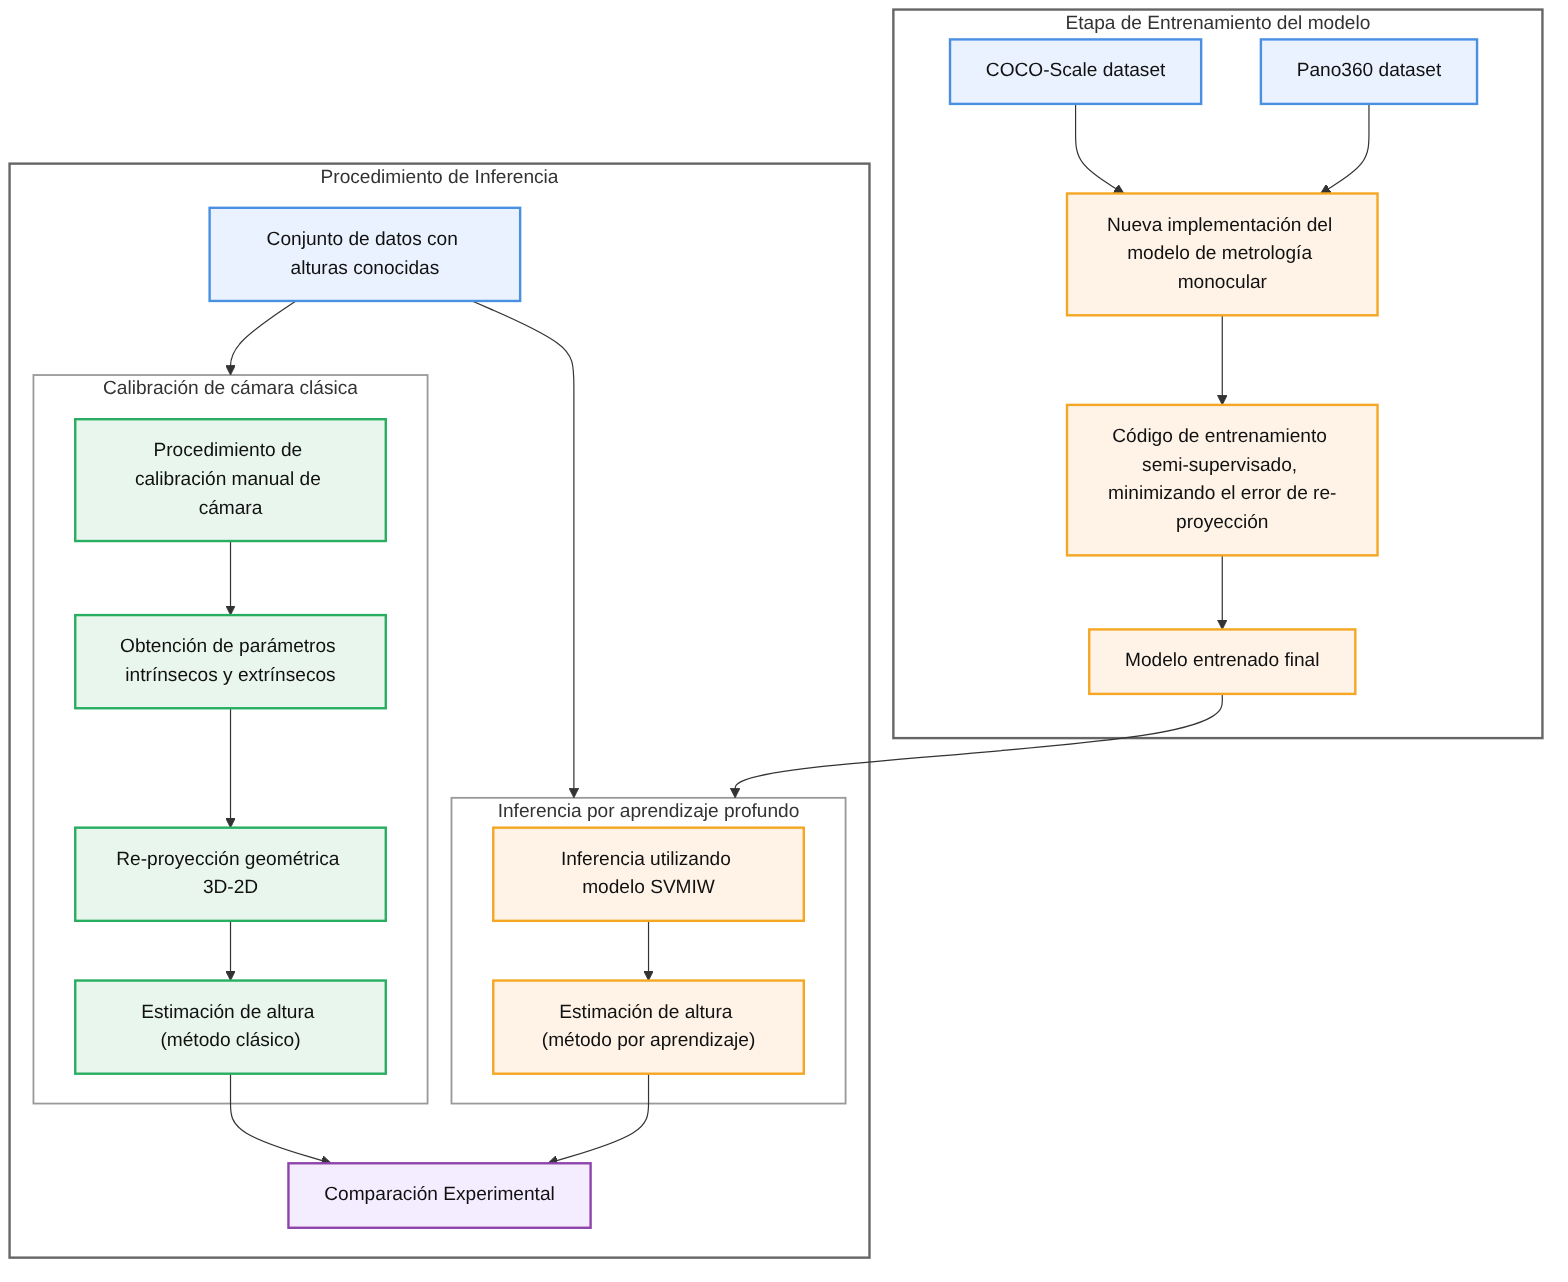
\includegraphics[width=1\textwidth]{imagenes/chapter5/diagram}
%   \caption[Visualización del procedimiento experimental.]{
%   Visualización del procedimiento experimental.
%   Se entrena un modelo de aprendizaje profundo capaz de estimar la
%   altura de objetos y se compara sus predicciones frente al método de calibración manual de cámara y reproyección geométrica.
% }\label{fig:Mermaid}
% \end{figure}

\section{Resultados método clásico}
En la Tabla~\ref{tab:ManualResults} se observan los resultados de
aplicar el método descrito en la Sección~\ref{sec:ManualCalibration},
de calibración manual de escena en IdentAI~\cite{panacea2026}.
En dicha tabla, se expresa el error medio ($\mu$), la desviación típica ($\sigma$), la varianza ($\sigma^2$), la mediana,
el tercer cuartil ($Q_3$) y el error máximo. El tercer cuartil es una medida estadística que indica el valor
por debajo del cual se encuentra el 75\% de los datos ordenados de menor a mayor.
El error medio es de 6.7 centímetros para todas las cámaras.
Destaca la cámara 1 con el mayor error de estimación, con 41.6 centímetros,
y la mayor varianza, de 0.006 $m^2$. En el caso correspondiente a dicha estimación,
el individuo se encontraba en el borde de la imagen, región en la que los efectos
de la distorsión óptica de la cámara son más pronunciados (véase la Figura~\ref{fig:ManualWorst}).
Esta circunstancia podría explicar, al menos parcialmente, el carácter extremo de la estimación obtenida.
Por otro lado, en la Figura~\ref{fig:ManualBest} se observan los ejemplos
con una estimación coincidente.
\begin{table}[!ht]
  \centering
  \scriptsize
\begin{tabular}{|l|c|c|c|c|c|c|c|}
\hline
\rowcolor[HTML]{FFCB2F}
\textbf{Cámara} & \textbf{Soporte} & $\bm{\mu}$ & $\bm{\sigma}$ & $\bm{\sigma^2}$ & \textbf{Mediana} & $\bm{Q_3}$ & \textbf{Máximo} \\
\hline
Cam1 & 209 & 0.092 & 0.078 & 0.006 &0.070 & 0.134 & 0.416 \\
\hline
Cam2 & 277 & 0.052 & 0.038 & 0.001 &0.046 & 0.073 & 0.194 \\
\hline
Cam3 & 166 & 0.062 & 0.035 & 0.001 &0.063 & 0.087 & 0.149 \\
\hline
\textbf{Total} & \textbf{652} & \textbf{0.067} & \textbf{0.056} & \textbf{0.003} & \textbf{0.055} & \textbf{0.091} & \textbf{0.416} \\
\hline
\end{tabular}
\caption[Tabla de errores de estimación del método de calibración manual, expresados en metros.]{
 Tabla de errores de estimación del método de calibración manual, expresados en metros.
 Se observa que, en escenas con la cámara cuidadosamente calibrada y medidas de referencia precisas, el error medio de estimación de la altura de los
 individuos es relativamente bajo. Aún así, destaca la cámara 1 que obtuvo un error máximo de 41.6 centímetros.
}
\label{tab:ManualResults}
\end{table}

\begin{figure}[!ht]
  \centering
  \subfloat{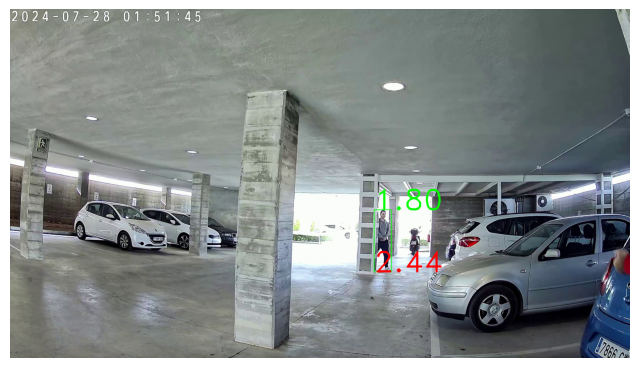
\includegraphics[width=0.5\textwidth]{imagenes/chapter5/worst_fail_cam1.png}}
  \subfloat{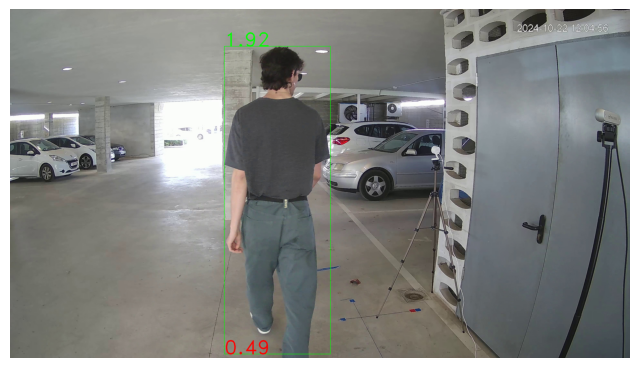
\includegraphics[width=0.5\textwidth]{imagenes/chapter5/worst_fail_cam2.png}}\\
  \subfloat{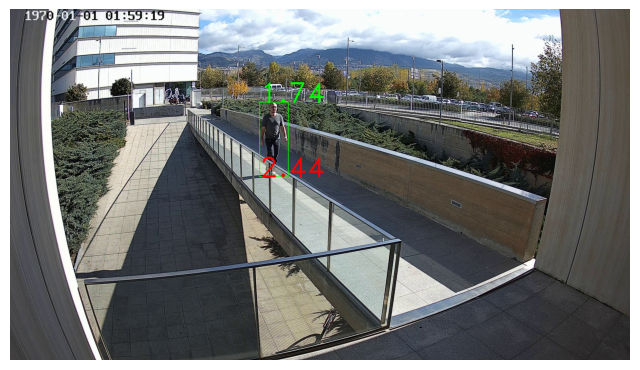
\includegraphics[width=0.5\textwidth]{imagenes/chapter5/worst_fail_cam3.png}}
  \caption[Visualización de las peores predicciones del método de calibración manual.]{
  Se observan ejemplos con las peores mediciones para cada cámara con el método de calibración manual, donde el número en color verde es el valor esperado y el de color rojo el estimado.
  En el ejemplo superior izquierdo, se obtiene un error absoluto de 42 centímetros tras estimar 2.22 metros de altura cuando el sujeto mide 1.80 metros.
  En el ejemplo superior derecho, el error absoluto es de 19 centímetros, con una estimación de 1.51 metros frente al valor real de 1.70 metros.
  Finalmente, el ejemplo inferior presenta un error absoluto de 15 centímetros, con una estimación de 1.77 metros frente al valor real de 1.92 metros.
}\label{fig:ManualWorst}
\end{figure}

\begin{figure}[H]
  \centering
  \subfloat{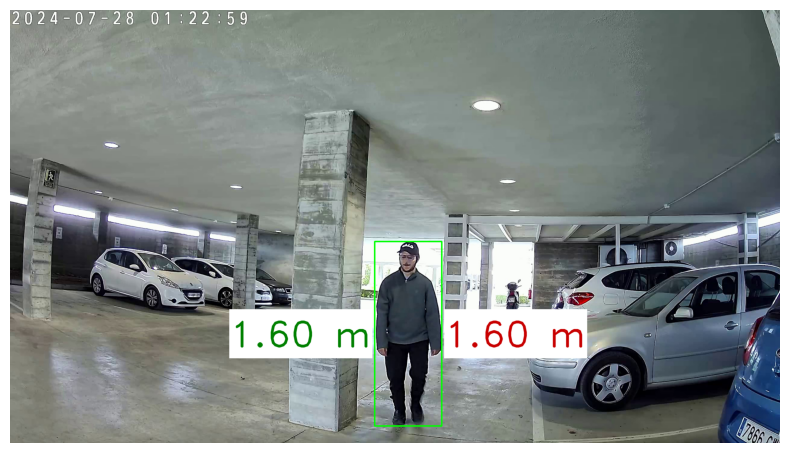
\includegraphics[width=0.5\textwidth]{imagenes/chapter5/perfect_cam1.png}}
  \subfloat{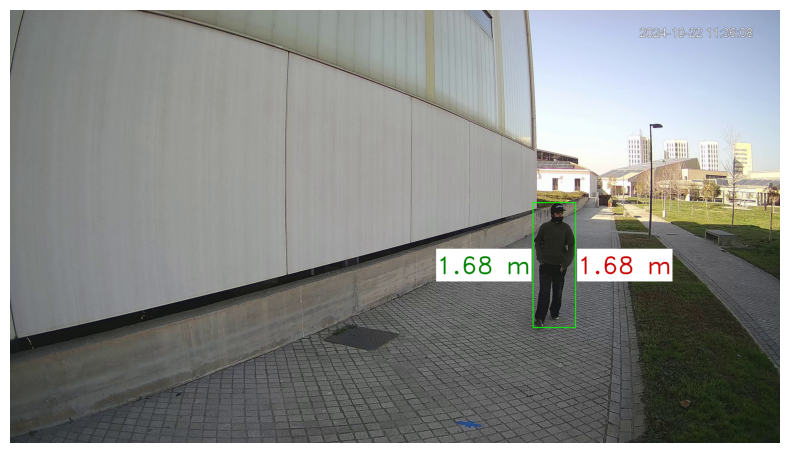
\includegraphics[width=0.5\textwidth]{imagenes/chapter5/perfect_cam2.png}}\\
  \subfloat{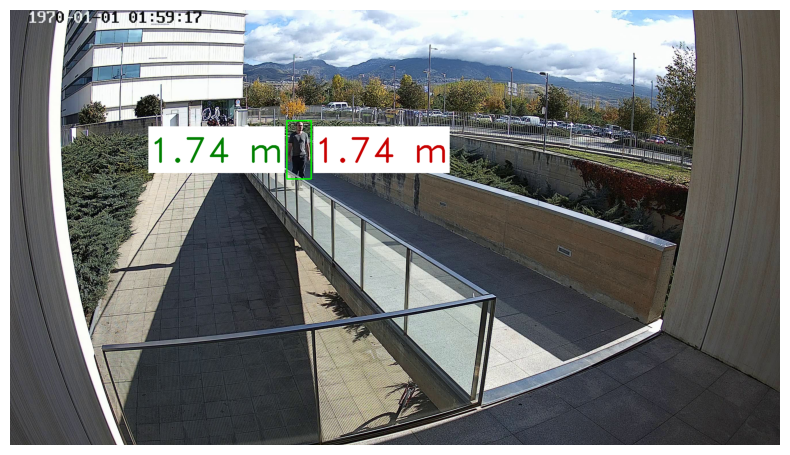
\includegraphics[width=0.5\textwidth]{imagenes/chapter5/perfect_cam3.png}}
  \caption[Visualización de predicciones coincidentes del método de calibración manual.]{
  Se observan ejemplos de mediciones coincidentes con cada cámara con el método de calibración manual, donde el número en color verde es el valor esperado y el de color rojo el estimado.
  En el ejemplo superior izquierdo, la altura real y la estimada coinciden en 1.60 metros.
  En el ejemplo superior derecho, ambas presentan un valor de 1.68 metros.
  Finalmente, en el ejemplo inferior, la altura real y estimada es de 1.74 metros.
}\label{fig:ManualBest}
\end{figure}


El método de calibración manual es susceptible a acumulación de errores por imprecisión en
diferentes pasos del proceso, ya sea por imprecisión de los parámetros estimados de la matriz de proyección
de la cámara, de su posición con relación al sujeto en escena o sus ángulos de rotación. En este caso, las imágenes
rectificadas no presentan anomalías evidentes. Por lo tanto, el peso del error recae sobre la calidad
de la estimación del recuadro delimitador (debe ser lo más acertado posible respecto a los pies y cabeza de los individuos),
y la precisión de la posición de la cámara (altura respecto al suelo, distancia al individuo y rotación).

Dado que los fotogramas están altamente relacionados, en una misma grabación, con el siguiente y, por lo tanto, el anterior, en la Tabla~\ref{tab:ManualResultsBySubject} se
recogen los valores medios de estimación por individuo y su error asociado.
No se observa un patrón evidente en el error correspondiente a una altura concreta.
El error absoluto promedio por individuo es de 5.8 centímetros, ligeramente inferior al error absoluto a nivel de fotograma de 6.7 centímetros.
Dado que las estimaciones presentan una baja varianza debido a la naturaleza del algoritmo y de los fotogramas obtenidos de las grabaciones,
es de esperar que errores elevados en sujetos con mayor cantidad de fotogramas lleven el promedio por fotograma a ser más pesimista
que al agrupar por individuo. Por otro lado, en la Tabla~\ref{tab:ManualResultsByScene}
se recogen los errores de las estimaciones agrupadas por tipo de escena.

\begin{table}[!ht]
  \scriptsize
  \centering
\begin{tabular}{|l|c|c|c|c|c|c|}
\hline
\rowcolor[HTML]{FFCB2F}
\textbf{Sujeto}&\textbf{ Soporte }&\textbf{ Altura }&\textbf{ Estimación media }& $\bm{\sigma}$ & $\bm{\sigma^2}$ &\textbf{ Error medio } \\
\hline
idai001 & 56 & 1.620 & 1.590 & 0.062 & 0.004 & 0.056 \\
\hline
idai002 & 77 & 1.600 & 1.588 & 0.109 & 0.012 & 0.076 \\
\hline
idai003 & 4 & 1.840 & 1.930 & 0.008 & 0.000 & 0.090 \\
\hline
idai006 & 90 & 1.800 & 1.770 & 0.094 & 0.009 & 0.070 \\
\hline
idai007 & 65 & 1.690 & 1.667 & 0.072 & 0.005 & 0.058 \\
\hline
idai008 & 51 & 1.750 & 1.675 & 0.039 & 0.002 & 0.080 \\
\hline
idai009 & 4 & 1.780 & 1.791 & 0.023 & 0.001 & 0.017 \\
\hline
idai010 & 131 & 1.920 & 1.850 & 0.057 & 0.003 & 0.077 \\
\hline
idai011 & 6 & 1.740 & 1.727 & 0.019 & 0.000 & 0.021 \\
\hline
idai012 & 78 & 1.700 & 1.652 & 0.105 & 0.011 & 0.096 \\
\hline
idai014 & 49 & 1.740 & 1.749 & 0.027 & 0.001 & 0.024 \\
\hline
idai015 & 41 & 1.680 & 1.684 & 0.043 & 0.002 & 0.032 \\
\hline
\end{tabular}
\caption[Tabla de errores de estimación del método de calibración manual por individuo, expresados en metros.]{
  Tabla de errores de estimación del método de calibración manual por individuo, expresados en metros.
  Se observa un error absoluto reducido para todos los sujetos, lo que evidencia la capacidad
  de estimación del método cuando se dispone de una calibración de cámara precisa y mediciones rigurosas de la escena.
}\label{tab:ManualResultsBySubject}
\end{table}

\begin{table}[!ht]
  \centering
  \scriptsize
\begin{tabular}{|l|c|c|c|c|c|c|c|}
\hline
\rowcolor[HTML]{FFCB2F}
\textbf{Escena} & \textbf{Soporte} & $\bm{\mu}$ & $\bm{\sigma}$ & $\bm{\sigma^2}$ & \textbf{Mediana} & $\bm{Q_3}$ & \textbf{Máximo} \\
\hline
Aparcamiento & 428 & 0.074 & 0.064 & 0.004 &0.056 & 0.101 & 0.416 \\
\hline
Rampa & 155 & 0.062 & 0.035 & 0.001 &0.064 & 0.088 & 0.149 \\
\hline
Sala de seminarios & 28 & 0.045 & 0.028 & 0.001 &0.040 & 0.061 & 0.099 \\
\hline
Acera & 41 & 0.032 & 0.028 & 0.001 &0.021 & 0.046 & 0.127 \\
\hline
\end{tabular}
\caption[Tabla de errores de estimación del método de calibración manual por escena, expresados en metros.]{
  Tabla de errores de estimación del método de calibración manual por escena, expresados en metros.
  Destaca la escena del aparcamiento, con un error máximo de 41.6 centímetros. Por otro lado, en la sala
  de seminarios se obtienen el menor error máximo, con tan solo 9.9 centímetros.
}
\label{tab:ManualResultsByScene}
\end{table}

A modo de comparación, en la Tabla~\ref{tab:BaselineDummy} se muestran
los errores medios de utilizar otro modelo de referencia. Se trata del método estático, que predice siempre la altura media de 1.75 metros.
El error medio de dicho método es de 8.8 centímetros. Por lo tanto, el método de estimación por calibración de la escena
permite obtener estimaciones más precisas que simplemente utilizar el valor medio de altura.
No obstante, el método de calibración manual depende de mediciones rigurosas de la escena, así como el uso
de un proceso de calibración de cámara extenso, para lograr errores de estimación aceptables. Escenas posiblemente mal calibradas
o cuyas medidas de referencia no sean precisas pueden dar lugar a valores extremos de estimación, como el error máximo de 41.6 centímetros.

\begin{table}[!ht]
  \centering
  \scriptsize
\begin{tabular}{|l|c|c|c|c|c|c|c|}
\hline
\rowcolor[HTML]{FFCB2F}
\textbf{Cámara} & \textbf{Soporte} & $\bm{\mu}$ & $\bm{\sigma}$ & $\bm{\sigma^2}$ & \textbf{Mediana} & $\bm{Q_3}$ & \textbf{Máximo} \\
\hline
Cam1 & 209 & 0.098 & 0.053 & 0.003 &0.060 & 0.150 & 0.170 \\
\hline
Cam2 & 277 & 0.094 & 0.048 & 0.002 &0.070 & 0.150 & 0.170 \\
\hline
Cam3 & 166 & 0.066 & 0.077 & 0.006 &0.010 & 0.170 & 0.170 \\
\hline
\textbf{Total} & \textbf{652} & \textbf{0.088} & \textbf{0.060} & \textbf{0.004} & \textbf{0.060} & \textbf{0.150} & \textbf{0.170} \\
\hline
\end{tabular}
\caption[Tabla de errores de estimación del estimador estático, expresados en metros.]{
  Tabla de errores de estimación del estimador estático, expresados en metros.
  Se observan los errores medios del método que predice siempre la altura media de 1.75 metros.
}
\label{tab:BaselineDummy}
\end{table}

\section{Resultados método por aprendizaje profundo}
Para el entrenamiento del modelo se utilizó una tasa de aprendizaje extraída de~\cite{goyal2018accuratelargeminibatchsgd},
con un planificador para reducir su valor conforme se acerca al número total de iteraciones programadas,
con un recorte del gradiente según la norma L2 (para evitar divergencias durante el entrenamiento provocadas por conjuntos de ejemplos
ruidosos) y se opta por utilizar el mayor número de imágenes por iteraciones que permita
el hardware disponible. Debido a la alta demanda de uso de los servidores, se ha utilizado
una única tarjeta de cómputo de 12GB de VRAM y, por lo tanto, la mitad de número de ejemplos de entrenamiento
por iteración en comparación al artículo de referencia~\cite{SVMIW}.
\par
El entrenamiento se realiza en tres fases, como se describe en la Sección~\ref{sec:AutoMethod}.
La primera entrena solamente la estimación de los parámetros de la cámara mientras mantiene las capas iniciales,
de extracción de características generales, congeladas para no afectar a la capacidad del modelo de detectar personas.
La segunda, entrena conjuntamente la estimación de parámetros de la cámara y la detección de personas, para alinear el
modelo al tipo de persona que se debe detectar. En concreto, se debe detectar solamente personas totalmente visibles y que se
encuentren con los pies en el suelo. Es decir, se debe restringir la capacidad del modelo generalista, de detección de personas,
a este subconjunto de personas que cumplen estas restricciones geométricas para la estimación de su estatura.
Finalmente, se añaden las últimas capas y la función de pérdida para la estimación de la altura del sujeto y de la cámara.
Todas las fases se entrenan por 30K iteraciones.
\par
En la Tabla~\ref{tab:CalibResults} se comparan los resultados obtenidos en esta implementación
con la tabla de resultados del artículo~\cite{SPEC}, que incluye los resultados del artículo de referencia~\cite{SVMIW},
sobre el conjunto de datos Pano360. Se evidencia la capacidad de esta implementación de replicar, e incluso superar,
la precisión obtenida en algunas métricas de las referencias, con un menor número de ejemplos procesados.
En términos de número total de ejemplos de calibración vistos, se observan 33 veces menos ejemplos que~\cite{SPEC} y 1.78 veces menos que~\cite{SVMIW}.
Se incluyen también los resultados del modelo final, una vez entrenado sobre todas las fases, y se observa
que su capacidad de estimar los parámetros de la cámara no diverge tanto del modelo entrenado solamente para
ello. De hecho, su capacidad de estimar el ángulo de visión vertical (\emph{vfov}) y el de inclinación (\emph{pitch})
mejora ligeramente frente a dicho modelo.
Esto podría deberse a que el modelo en la fase final tiene acumulado más iteraciones totales, así como
la presencia de la restricción proyectiva de la estimación de la altura del sujeto que afecta a las predicciones
de los ángulos de la cámara.

\begin{table}[!ht]
  \centering
  \scriptsize
  \begin{tabular}{|l|c|c|c|}
  \hline
  \rowcolor[HTML]{FFCB2F}
  \textbf{Método} & \textbf{VFOV ($^\circ$)$\downarrow$} & \textbf{Pitch ($^\circ$)$\downarrow$} & \textbf{Roll ($^\circ$)$\downarrow$} \\
  \hline
  ScaleNet~\cite{SVMIW} & 5.68 & 2.61 & 1.41 \\
  \hline
  CamCalib (KL Loss)~\cite{SPEC} & 3.53 & 2.32 & 1.15 \\
  \hline
  CamCalib (Softargmax-L2)~\cite{SPEC} & 3.34 & 2.06 & 1.11 \\
  \hline
  CamCalib (Softargmax-biased-L2)~\cite{SPEC} & \textbf{3.24} & \textbf{1.94} & 1.02 \\
  \hline
  Modelo entero fase 0 (Softargmax-biased-L2) & 3.98 & 2.43 & \textbf{0.89} \\
  \hline
  Solo clasificadores fase 0 (Softargmax-biased-L2) & 6.09 & 3.78 & 1.54 \\
  \hline
  Modelo fase final (Softargmax-biased-L2) & 3.46 & 2.34 & 1.05 \\
  \hline
  \end{tabular}
  \caption[Tabla comparativa de la precisión de la estimación de los parámetros de la cámara en Pano360~\cite{SPEC}.]
  {
    Tabla comparativa de la precisión de la estimación de los parámetros de la cámara en Pano360~\cite{SPEC}.
    Los resultados de los cuatro primeros métodos son extraídos de~\cite{SPEC}. Aunque no se tiene la partición exacta en la que se
    evaluaron los demás modelos, se utiliza la misma proporción de ejemplos de validación (3.6\%) con un total de 12.732 imágenes (ligeramente inferior a las 15K utilizadas en~\cite{SPEC}),
    obtenidas mediante el mismo código de generación de las particiones de entrenamiento y validación de~\cite{SPEC}.
    La implementación actual demuestra ser capaz de competir contra los resultados de las implementaciones de referencia,
    con el modelo entero entrenado (solo en la fase 0)
    viendo en total hasta 33 veces menos ejemplos que CamCalib~\cite{SPEC}, y 1.78 veces menos que ScaleNet~\cite{SVMIW}
}\label{tab:CalibResults}
\end{table}

En la Tabla~\ref{tab:vt_losses} se compara el error de
reproyección obtenido en el conjunto de test de COCO-Scale, así como en el conjunto de KITTI-person.
Se observa que el error de reproyección es idéntico en el conjunto de COCO-Scale y, aunque ligeramente diferente en el KITTI-person,
el error de medición en KITTI-person es inferior.
En este último, aunque no se disponga de la misma partición de datos que los autores de referencia~\cite{SVMIW},
la partición utilizada contiene 1352 imágenes frente a las 298 imágenes utilizadas por los mismos.
Aunque las particiones no son directamente comparables, los resultados obtenidos muestran que la implementación
presenta un comportamiento competitivo bajo la partición utilizada.

\begin{table}[!ht]
  \centering
  \scriptsize
  \begin{tabular}{|l|c|c|c|}
  \hline
  \rowcolor[HTML]{FFCB2F}
  \textbf{Dataset} & \textbf{Método} & \textbf{Error de reproyección} & \textbf{Error de medición}\\
  \hline
  \multirow{2}{*}{COCO-Scale} & ScaleNet SN-L3~\cite{SVMIW} & 0.07 & -\\
  \cline{2-4}
                                     & Nuestro & 0.07 & - \\
  \hline
  KITTI-person & ScaleNet SN-L3~\cite{SVMIW} & 0.03 & 0.10 metros\\
  \hline
  KITTI-person* & Nuestro & 0.04 & 0.09 metros\\
  \hline
  \end{tabular}
  \caption[Tabla comparativa de error de reproyección obtenido.]{
  Tabla comparativa de error de reproyección obtenido.
  Se observa que el modelo muestra un comportamiento comparable al de referencia, obteniendo valores
  muy cercanos en las particiones utilizadas. Todo ello con 70K iteraciones menos, utilizando la mitad de ejemplos
  por cada. La partición utilizada de KITTI-person* no es exactamente igual al del artículo~\cite{SVMIW}.
  En este caso, se incluyen muchas más imágenes, con un total de 1352 frente a 298.
  Aun así, se logra obtener un error medio de altura ligeramente inferior.

}\label{tab:vt_losses}
\end{table}
En la Tabla~\ref{tab:AutoResults}
se observan los resultados del método de estimación automática en IdentAI~\cite{panacea2026}. El error medio de
las cámaras en conjunto es de 9.8 centímetros, se encuentra en el mismo orden de magnitud que método de calibración manual de escena.
Un error cercano al método de estimación estática de altura media, pero logrando permitir la estimación de la
altura exacta de individuos cuya altura no es 1.75 metros en diversas escenas.
Los valores de mediana y tercer cuartil también son cercanos al método de calibración manual, dejando ver lo prometedor que podría llegar a ser este método.
Destacan los valores máximos que no llegan a sobrepasar los 33 centímetros de error, mientras que el método de calibración manual ha llegado a tener
un error de 41.6 centímetros (valor atípico, un error extremo de estimación de altura por retroproyección).
Por otro lado, en la Tabla~\ref{tab:ResultsBySubject} se observa cómo se
comporta el método por cada sujeto del estudio y se destaca que el modelo parece tener dificultades
para estimar valores lejanos al ~\emph{a priori} de 1.75 metros para las escenas estudiadas.
El error promedio agrupado por individuo es de 7.4 centímetros, cercano a los 5.8 centímetros del método
de calibración manual y los 6.8 centímetros del método de predicción estática.
No obstante, el modelo parece subestimar las alturas para sujetos con altura superior a 1.75, mientras
que realiza sobreestimaciones sobre sujetos con estatura inferior a dicho valor. En otras palabras,
el modelo presenta un efecto de regresión hacia la media, consistente con la presencia del prior
antropométrico introducido durante el entrenamiento (véase la Figura~\ref{fig:AutoHeightDist}).
Un ajuste equilibrado de los pesos de la combinación
lineal de pérdidas podría ayudar a evitar este efecto. De otra forma, controlar la tasa de
aprendizaje de la capa de estimación de altura, así como la magnitud del gradiente que le afecta, podría ayudar a
regularizar este comportamiento.

\begin{figure}[!ht]
  \begin{center}
    \subfloat{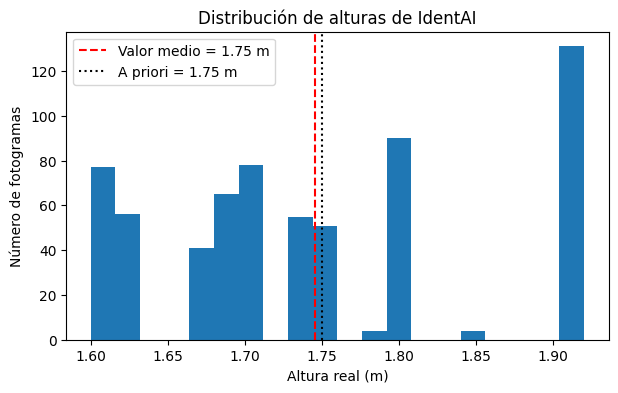
\includegraphics[width=0.5\textwidth]{imagenes/chapter5/svimw_height_dist.png}}
    \subfloat{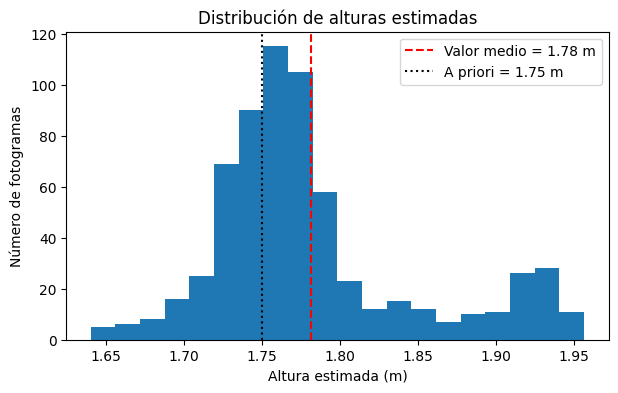
\includegraphics[width=0.5\textwidth]{imagenes/chapter5/svimw_pred_height_dist.png}}
  \end{center}
  \caption[Distribución de predicciones de altura del modelo por aprendizaje profundo.]{
  Distribución de predicciones de altura del modelo por aprendizaje profundo.
  Se observa un efecto de regresión hacia el~\emph{a priori} de 1.75 metros, obteniendo un valor promedio de
  estimaciones de 1.78 metros. El efecto provoca que el modelo tienda a realizar
  sobreestimaciones para sujetos de pequeña estatura y subestimaciones para sujetos de gran estatura.
}\label{fig:AutoHeightDist}
\end{figure}


\begin{table}[!ht]
  \centering
  \scriptsize
\begin{tabular}{|l|c|c|c|c|c|c|c|}
\hline
\rowcolor[HTML]{FFCB2F}
\textbf{Cámara} & \textbf{Soporte} & $\bm{\mu}$ & $\bm{\sigma}$ & $\bm{\sigma^2}$ & \textbf{Mediana} & $\bm{Q_3}$ & \textbf{Máximo} \\
\hline
Cam1 & 209 & 0.121 & 0.082 & 0.007 &0.120 & 0.173 & 0.328 \\
\hline
Cam2 & 277 & 0.094 & 0.051 & 0.003 &0.077 & 0.141 & 0.210 \\
\hline
Cam3 & 166 & 0.074 & 0.068 & 0.005 &0.038 & 0.147 & 0.203 \\
\hline
\textbf{Total} & \textbf{652} & \textbf{0.098} & \textbf{0.069} & \textbf{0.005} & \textbf{0.081} & \textbf{0.152} & \textbf{0.328} \\
\hline
\end{tabular}
\caption[Tabla de errores de estimación del método por aprendizaje profundo, expresados en metros.]{
  Tabla de errores de estimación del método por aprendizaje profundo, expresados en metros.
  Se observan resultados prometedores del método de estimación automática por aprendizaje.
  Destaca el error medio de la cámara 3, que podría estar relacionado con su mejor calidad de imagen.}
\label{tab:AutoResults}
\end{table}

\begin{table}[H]
  \scriptsize
  \centering
\begin{tabular}{|l|c|c|c|c|c|c|}
\hline
\rowcolor[HTML]{FFCB2F}
\textbf{Sujeto}&\textbf{ Soporte }&\textbf{ Altura }&\textbf{ Estimación media }&$\bm{\sigma}$&$\bm{\sigma^2}$ &\textbf{ Error medio }\\
\hline
idai001 & 56 & 1.620 & 1.771 & 0.045 & 0.002 & 0.151 \\
\hline
idai002 & 77 & 1.600 & 1.788 & 0.051 & 0.003 & 0.188 \\
\hline
idai003 & 4 & 1.840 & 1.852 & 0.036 & 0.001 & 0.031 \\
\hline
idai006 & 90 & 1.800 & 1.829 & 0.074 & 0.005 & 0.066 \\
\hline
idai007 & 65 & 1.690 & 1.786 & 0.049 & 0.002 & 0.096 \\
\hline
idai008 & 51 & 1.750 & 1.750 & 0.025 & 0.001 & 0.021 \\
\hline
idai009 & 4 & 1.780 & 1.767 & 0.010 & 0.000 & 0.013 \\
\hline
idai010 & 131 & 1.920 & 1.801 & 0.069 & 0.005 & 0.123 \\
\hline
idai011 & 6 & 1.740 & 1.756 & 0.006 & 0.000 & 0.016 \\
\hline
idai012 & 78 & 1.700 & 1.794 & 0.061 & 0.004 & 0.094 \\
\hline
idai014 & 49 & 1.740 & 1.704 & 0.024 & 0.001 & 0.036 \\
\hline
idai015 & 41 & 1.680 & 1.724 & 0.029 & 0.001 & 0.049 \\
\hline
\end{tabular}
\caption[Tabla de errores de estimación del método por aprendizaje profundo por individuo, expresados en metros.]{
Tabla de errores de estimación del método por aprendizaje profundo por individuo, expresados en metros.
Se observa que el modelo parece tener dificultades a la hora de estimar correctamente la altura para los individuos
cuya estatura es lejana al \emph{a priori} de 1.75.
}\label{tab:ResultsBySubject}
\end{table}

Dado que se conoce la altura de la cámara en las escenas,
se pueden ver reflejados en la Tabla~\ref{tab:AutoCamResults}
el error medio de estimación del módulo de PointNet~\cite{PointNet} de la altura de la cámara.
Realizar un entrenamiento más largo del modelo puede que reduzca la varianza y el error obtenido,
tanto en la estimación de la altura de la cámara como del sujeto en escena.
El error medio agrupado por escena de la estimación de la altura de la cámara es de 10.5 centímetros.
En la Tabla~\ref{tab:AutoCamResultsByScene} se observa que el modelo parece tener dificultades para
realizar estimaciones acertadas en la escena del aparcamiento.
Aún así, incluso con el error de estimación de la altura de la cámara en dicha escena, se observan
ejemplos en la misma con predicciones coincidentes. Esto podría deberse a que existen diversas soluciones de la
combinación de las estimaciones (rotación de la cámara, distancia al objeto, altura del objeto y de la cámara)
que podrían llevar a un mismo error de reproyección. Por lo tanto, un error bajo de reproyección
no garantiza que los parámetros geométricos estimados sean físicamente correctos. Esta es una
limitación identificada del modelo y, para poder resolverla, sería necesario
encontrar una restricción adicional sobre la escena.

\begin{table}[!ht]
  \centering
  \scriptsize
\begin{tabular}{|l|c|c|c|c|c|c|c|}
\hline
\rowcolor[HTML]{FFCB2F}
\textbf{Cámara} & \textbf{Soporte} & $\bm{\mu}$ & $\bm{\sigma}$ & $\bm{\sigma^2}$ & \textbf{Mediana} & $\bm{Q_3}$ & \textbf{Máximo} \\
\hline
Cam1 & 209 & 0.295 & 0.102 & 0.010 &0.323 & 0.361 & 0.421 \\
\hline
Cam2 & 277 & 0.161 & 0.077 & 0.006 &0.172 & 0.212 & 0.399 \\
\hline
Cam3 & 166 & 0.065 & 0.041 & 0.002 &0.059 & 0.091 & 0.183 \\
\hline
\textbf{Total} & \textbf{652} & \textbf{0.179} & \textbf{0.118} & \textbf{0.014} & \textbf{0.169} & \textbf{0.285} & \textbf{0.421} \\
\hline
\end{tabular}
\caption[Tabla de errores de estimación de la altura de la cámara con aprendizaje automático, expresados en metros.]{
  Tabla de errores de estimación de la altura de la cámara con aprendizaje automático, expresados en metros.
  Debido a que los datos de entrada a este módulo son estimaciones anteriores, existe una propagación de errores que podría dar lugar a predicciones más ruidosas.
}
\label{tab:AutoCamResults}
\end{table}

\begin{table}[!ht]
  \centering
  \scriptsize
\begin{tabular}{|l|c|c|c|c|c|c|c|}
\hline
\rowcolor[HTML]{FFCB2F}
\textbf{Escena} & \textbf{Soporte} & $\bm{\mu}$ & $\bm{\sigma}$ & $\bm{\sigma^2}$ & \textbf{Mediana} & $\bm{Q_3}$ & \textbf{Máximo} \\
\hline
Aparcamiento & 428 & 0.242 & 0.095 & 0.009 &0.233 & 0.323 & 0.421 \\
\hline
Rampa & 155 & 0.060 & 0.036 & 0.001 &0.055 & 0.085 & 0.180 \\
\hline
Sala de seminarios & 28 & 0.065 & 0.041 & 0.002 &0.072 & 0.098 & 0.129 \\
\hline
Acera & 41 & 0.054 & 0.056 & 0.003 &0.036 & 0.064 & 0.183 \\
\hline
\end{tabular}
\caption[Tabla de errores de estimación de la altura de la cámara con aprendizaje automático por escena, expresados en metros.]{
Tabla de errores de estimación de la altura de la cámara con aprendizaje automático por escena, expresados en metros.
Se observa que el modelo parece tener problemas para realizar estimaciones en el aparcamiento,
obteniendo un error medio en la estimación de la altura de cámara de 24.2 centímetros, con error máximo en 42.1 centímetros.
}\label{tab:AutoCamResultsByScene}
\end{table}

En la Tabla~\ref{tab:Results} se recogen los resultados finales
de todos los métodos implementados.
Se observa que el método de aprendizaje profundo evita estimaciones extremas, reduciendo así
los errores máximos observables. Se aproxima al método de estimación estática (de 1.75 metros), con el beneficio de acertar en múltiples escenas
la estatura de diferentes sujetos. En las Figuras~\ref{fig:AutoWorst} y~\ref{fig:AutoBest} se
observan las peores y mejores estimaciones.

\begin{table}[H]
  \scriptsize
  \begin{center}
    \begin{tabular}{|l|c|c|c|c|c|c|c|}
      \rowcolor[HTML]{FFCB2F}
      \hline
      \textbf{Método} & $\bm{\mu}$ & $\bm{\sigma}$ & $\bm{\sigma^2}$ & \textbf{Mediana} & $\bm{Q_3}$ & \textbf{Máximo}\\
      \hline
      Estático (1.75 metros) & 0.088 & 0.060 & 0.004 & 0.060 & 0.150 & \textbf{0.170} \\
      \hline
      Calibración Manual & \textbf{0.067} & \textbf{0.056} & \textbf{0.003} & \textbf{0.055} & \textbf{0.091} & 0.416 \\
      \hline
      Nuestro & \textbf{0.098} & \textbf{0.069} & \textbf{0.005} & \textbf{0.081} & \textbf{0.152} & \textbf{0.328} \\
      \hline
    \end{tabular}
  \end{center}
  \caption[Tabla resumen de comparativa final, con errores expresados en metros.]{
  Tabla resumen de comparativa final, con errores expresados en metros.
  Se observa que incluir un \emph{a priori} sobre las estimaciones mejora el error máximo
  frente al método de calibración manual.
  No obstante, la baja variabilidad antropométrica de los datos (distribución de estatura muy centrada en 1.75), junto
  a errores de estimaciones elevados en algunas escenas (posibles problemas de aprendizaje del modelo), hace que el método de estimación estática
  del valor de altura medio (1.75 metros) presente un menor error medio. Aún así, dichos resultados se alcanzan de forma semi-supervisada y con un bajo número de iteraciones,
  indicando el potencial que posee dicho método de cara a automatizar y facilitar la estimación de la altura en entornos no controlados.
}\label{tab:Results}
\end{table}

\begin{figure}[H]
  \centering
  \subfloat{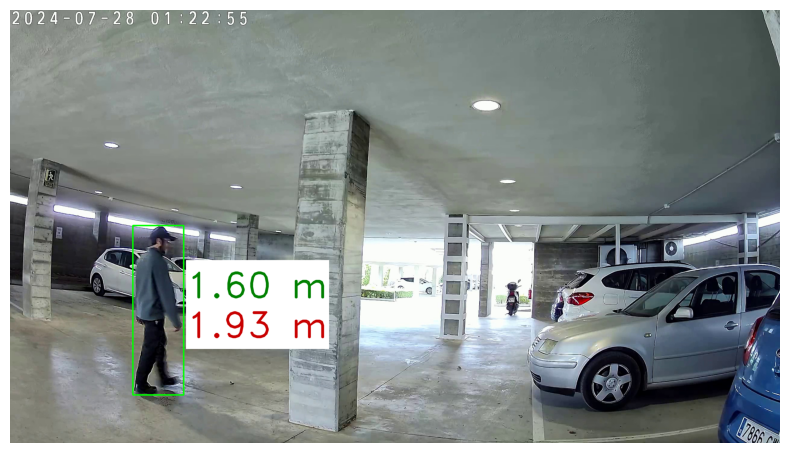
\includegraphics[width=0.5\textwidth]{imagenes/chapter5/worst_fail_cam1_svmiw.png}}
  \subfloat{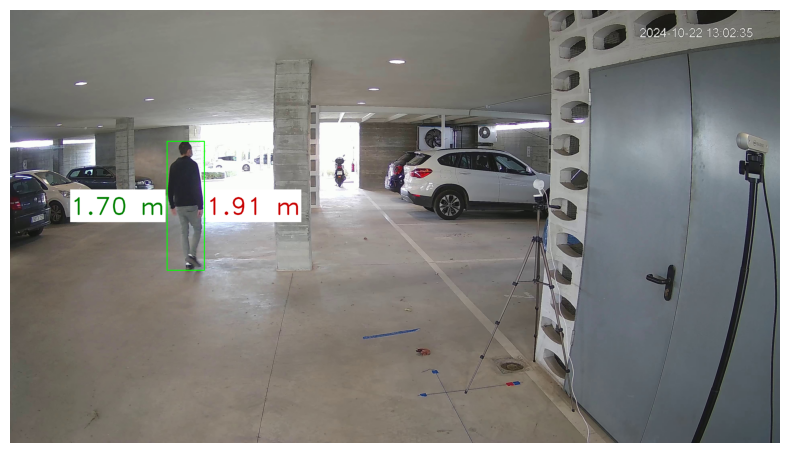
\includegraphics[width=0.5\textwidth]{imagenes/chapter5/worst_fail_cam2_svmiw.png}}\\
  \subfloat{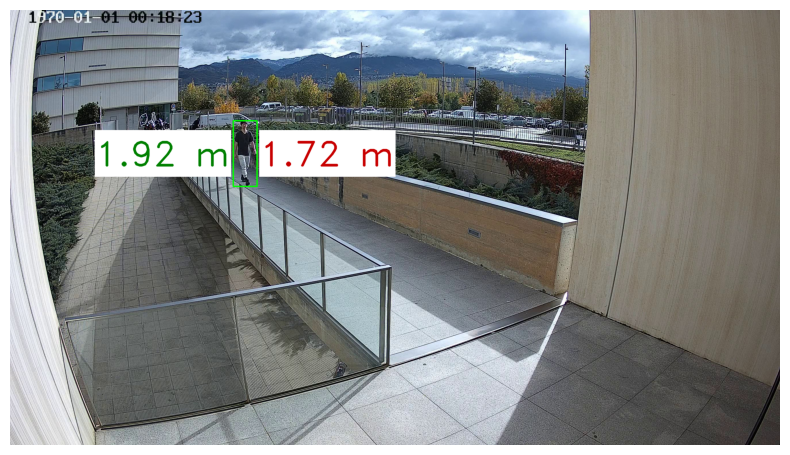
\includegraphics[width=0.5\textwidth]{imagenes/chapter5/worst_fail_cam3_svmiw.png}}
  \caption[Visualización de las peores predicciones del método por aprendizaje profundo.]{
  Se observan ejemplos con las peores mediciones para cada cámara con el método automático, donde el número en color verde es el valor esperado y el de color rojo el estimado.
  En el ejemplo superior izquierdo, se obtiene un error absoluto de 33 centímetros tras estimar 1.93 metros de altura cuando el sujeto mide 1.60 metros.
  En el ejemplo superior derecho, el error absoluto es de 21 centímetros, con una estimación de 1.91 metros frente al valor real de 1.70 metros.
  Finalmente, el ejemplo inferior presenta un error absoluto de 20 centímetros, con una estimación de 1.72 metros frente al valor real de 1.92 metros.
}
\label{fig:AutoWorst}
\end{figure}

\begin{figure}[H]
  \centering
  \subfloat{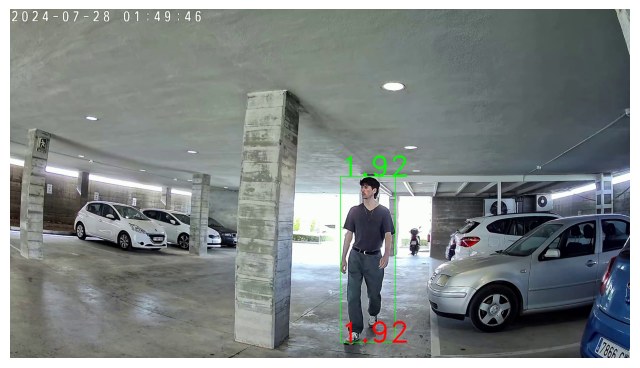
\includegraphics[width=0.5\textwidth]{imagenes/chapter5/perfect_cam1_svmiw.png}}
  \subfloat{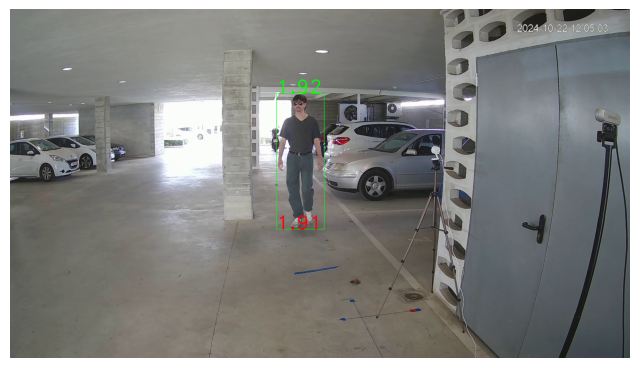
\includegraphics[width=0.5\textwidth]{imagenes/chapter5/perfect_cam2_svmiw.png}}\\
  \subfloat{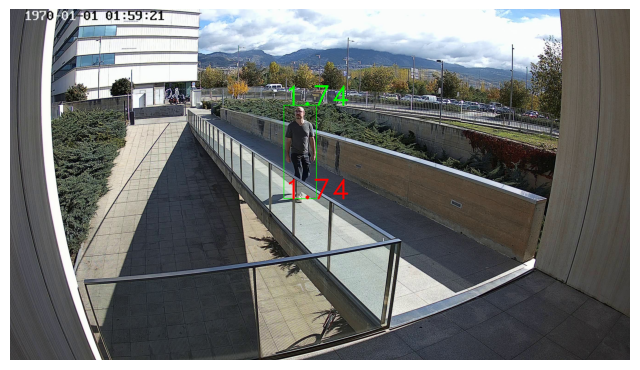
\includegraphics[width=0.5\textwidth]{imagenes/chapter5/perfect_cam3_svmiw.png}}
  \caption[Visualización de predicciones coincidentes con el método por aprendizaje profundo.]{
  Se observan ejemplos de mediciones coincidentes con cada cámara con el método automático, donde el número en color verde es el esperado y el de color rojo el estimado.
  En el ejemplo superior izquierdo, la altura real y la estimada coinciden en 1.92 metros.
  En el ejemplo superior derecho, ambas presentan un valor de 1.80 metros.
  Finalmente, en el ejemplo inferior, la altura real y estimada es de 1.75 metros.
  }
\label{fig:AutoBest}
\end{figure}
